\documentclass[11pt, oneside]{article}   	% use "amsart" instead of "article" for AMSLaTeX format
\usepackage{geometry}                		% See geometry.pdf to learn the layout options. There are lots.
\geometry{letterpaper}                   		% ... or a4paper or a5paper or ... 
\usepackage{graphicx}				% Use pdf, png, jpg, or eps§ with pdflatex; use eps in DVI mode
								% TeX will automatically convert eps --> pdf in pdflatex		
\usepackage{amssymb}
\usepackage{amsmath}
\usepackage{parskip}
\usepackage{color}
\usepackage{hyperref}

\graphicspath{{/Users/telliott_admin/Dropbox/Tex/png/}}
% \begin{center} 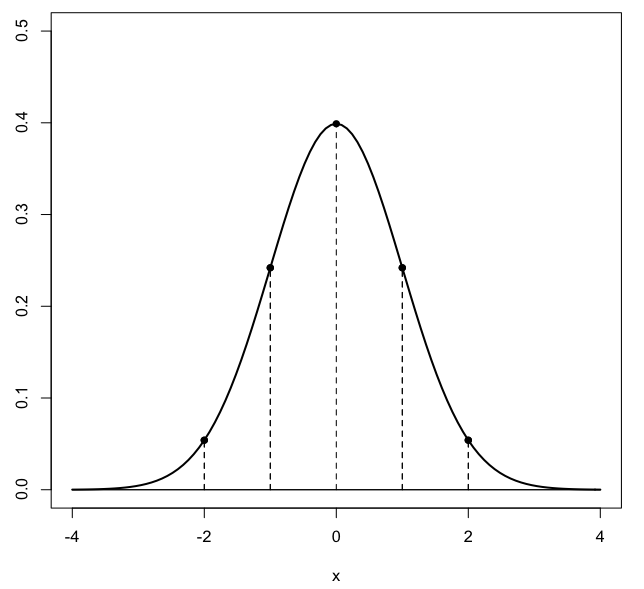
\includegraphics [scale=0.4] {gauss3.png} \end{center}

%break
\title{References}
\date{}

\begin{document}
\maketitle
\Large

$\bullet$ Auroux.  \emph{Multivariable Calculus}

\url{https://ocw.mit.edu/courses/mathematics/18-02-multivariable-calculus-fall-2007/}

$\bullet$ Acheson.  \emph{The Calculus Story}.

$\bullet$ Adams, Thompson, Hass. \emph{How to Ace the Rest of Calculus}.

$\bullet$ Alcock. \emph{Mathematics Rebooted}.

$\bullet$ Banner. \emph{The Calculus Lifesaver}.

$\bullet$ Colley. \emph{Vector Calculus}.

$\bullet$ Corral. \emph{Vector Calculus}.

$\bullet$ Courant, Robbins, Stewart. \emph{What is Mathematics?}.

$\bullet$ Dunham. \emph{Euler:  The Master of Us All}.

$\bullet$ Dunham. \emph{Journey Through Genius}.

$\bullet$ Dunham. \emph{The Mathematical Universe}.

$\bullet$ Feynman. \emph{The Character of Physical Law}.

$\bullet$ Fowler, Snapp. \emph{Mooculus}.

$\bullet$ Goodstein, Goodstein. \emph{Feynman's Lost Lecture}.

$\bullet$ Hamming.  \emph{Methods of Mathematics Applied to Calculus, Probability, and Statistics}.

$\bullet$ Kline. \emph{Calculus}.

$\bullet$ Lockhart. \emph{Measurement}.

$\bullet$ Maor. \emph{e, the Story of a Number}.

$\bullet$ Maor. \emph{To Infinity and Beyond}.

$\bullet$ Marsden, Tromba. \emph{Vector Calculus}.

$\bullet$ Morin. \emph{Probability}.

$\bullet$ Nahin. \emph{When least is best}.

$\bullet$ Savov. \emph{No bullshit guide to math and physics}.

\url{http://www.minireference.com}

$\bullet$ Schey.  \emph{Div, grad, curl}

$\bullet$ Shankar.  \emph{Fundamentals of Physics, vol I and II}.

$\bullet$ Spivak.  \emph{The Hitchhiker's Guide to Calculus}.

$\bullet$ Stewart.  \emph{Significant Figures}.

$\bullet$ Strang.  \emph{Calculus}.

$\bullet$ Strogatz.  \emph{The Joy of x}.

$\bullet$ Thompson.  \emph{Calculus Made Easy}.

$\bullet$ Varberg, Purcell, Rigdon.  \emph{Calculus with Differential Equations}.




\end{document}